%\documentclass[draft]{agujournal2018}
\documentclass[]{agujournal2018}
\usepackage{apacite}
\usepackage{url}
\usepackage{lineno}
%\linenumbers
\draftfalse
\journalname{Geophysical Research Letters}

%custom packages
\usepackage{amsmath,amssymb,amsfonts,amsthm}
\usepackage{comment}
\usepackage{booktabs}
% custom commands
\newcommand\be{\begin{equation}}
\newcommand\ee{\end{equation}} 
\newcommand\bra{\langle}
\newcommand\ket{\rangle}
\newcommand\om{\omega}
\newcommand\tom{\tilde{\omega}}
\newcommand\tg{\tilde{g}}
\newcommand\tp{\tilde{p}}
\newcommand\tG{\tilde{G}}
\newcommand\El{\mathcal{L}}
%\usepackage{layouts}
%\printinunitsof{in}\prntlen{\textwidth} % check scales in the document


\begin{document}

\title{Back to Einstein: how to include burial in fluvial sediment diffusion models?}

\authors{James K. Pierce \affil{1}and Marwan A. Hassan\affil{1}}
\affiliation{1}{Department of Geography \\University of British Columbia}
\correspondingauthor{James Kevin Pierce}{kpierce@alumni.ubc.ca}

\begin{keypoints}
\item We develop a random-walk model of objects in intermittent transport through an environment with traps
\item Its solution provides three ranges of diffusion, two of which are anomalous
\item We apply the model to sediment transport in rivers to clarify the scale-dependence of bedload diffusion

\end{keypoints}

\begin{abstract}
Sediment grains transport through gravel-bed rivers in cycles of motion and rest.
When grains rest on the surface, material transported from upstream can bury them.
Grains on the surface shield buried grains from the flow, so they can be immobile for long time periods.
These immobile periods can dominate sediment diffusion characteristics. 
Despite the significant impact of sediment burial on diffusion, existing models almost all neglect it.
In this letter, we present a random walk model incorporating sediment burial and solve it analytically.
The model predicts three sediment diffusion ranges with distinct scaling characteristics in each.
We relate the crossover times dividing these ranges to measurable transport parameters and describe each range from underlying physical processes.
Our developments provide new geophysical perspective on the scale-dependence of fluvial sediment transport.
\end{abstract}

\section{Introduction}

Anomalous diffusion has been subjected to intense research lately, as it emerges in contexts ranging from the transport of cholesterols through lipid bilayers \citep{Jeon2012,Molina-Garcia2018}, to contaminants through soils \citep{Berkowitz2006,Yang2019}, and pollinator insects through ecosystems \citep{Reynolds2009,Vallaeys2017}.
In this letter, we study anomalous diffusion in a river science context, where it emerges from coarse bedload sediment transporting through river channels \citep{Bradley2017,Martin2012,Ganti2010}.
Hans Albert Einstein developed the first model of bedload diffusion to describe his comprehensive experiments visually tracking painted grains through a flume \citep{Ettema2004,Einstein1937}.
Diffusion is the spreading apart of grains as they transport downstream, and it is induced by differences in the transport characteristics of one grain and the next.
Diffusion is usually quantified by the time dependence of the positional variance $\sigma_x^2(t)$ of a population.
When $\sigma_x^2 \propto t$, the diffusion is said to be normal, since this is found in the classic diffusion problems \citep[e.g.][]{Einstein1905,Taylor1920}.
However, many transport phenomena show $\sigma_x^2 \propto t^\gamma$ with $\gamma \neq 1$.
This diffusion is said to be anomalous \citep{Sokolov2012}. 
If $\gamma>1$, it is said to be super-diffusive; while if $\gamma <1$, it is said to be sub-diffusive \citep{Metzler2000}.
Einstein originally concluded that bedload transport expresses normal diffusion.

Researchers after Einstein have come to recognize that coarse sediment moving through river channels can show either anomalous or normal diffusion depending on the timescale of observation \citep{Nikora2002}.
This is a significant issue since it implies diffusion models should be scale dependent, and it renders experimental data contingent on their observation timescales.
\citet{Nikora2001a,Nikora2002} were the first to fundamentally rework Einstein's concept of bedload diffusion by introducing scale dependence.
They identified three ranges of diffusion from Newtonian simulations and experimental data, and they termed these ranges local, intermediate, and global in order of increasing timescale.
They determined that $\sigma_x^2$ scales with a different power of time in each range and concluded this scaling could be either anomalous or normal.
More recent works have more or less supported the Nikora et al. findings.
Various numerical approaches show two \citep[e.g.][]{Fan2016} or three \citep[e.g.][]{Bialik2012,Zhang2012} ranges of diffusion; one set of flume experiments appears to show two ranges of sediment diffusion \citep{Martin2012}, and several field studies have shown anomalous diffusion \citep{Bradley2017, Phillips2013}
However, the full picture of scale-dependent bedload diffusion is far from resolved.
In particular, we remain unclear on the diffusive scaling (super/normal/sub) of each range, and no model has been developed, to our knowledge, that derives all three diffusion ranges from process-based concepts of fluvial sediment transport.

In this letter, we develop a model of bedload diffusion that describes the local, intermediate, and global ranges of diffusion introduced by Nikora et al. by generalizing the original diffusion model of \citet{Einstein1937}.
Einstein has strongly influenced river geophysics and fostered an entire paradigm of research that leverages and generalizes his stochastic methods \citep[e.g.][]{Hubbell1964, Yano1969, Yang1971, Gordon1972, Nakagawa1976}.
His original model's essential content is that individual grains move in instantaneous steps interrupted by durations of rest which lie on statistical distributions \citep{Hassan1991}.
Einstein's model can be viewed as a special case of the continuous time random walk (CTRW) developed by \citet{Montroll1965} in condensed matter physics to describe the diffusion of charge carriers in solids.
Our generalization of Einstein's model has two components.
First, we include the duration and velocity of motions in place of instantaneous steps, and second, we add in the process of sediment burial, which has been associated with anomalous diffusion at long timescales \citep[e.g.][]{Bradley2017,Martin2014}.
To develop this generalization, we leverage the multi-state CTRW developed by \citet{Weiss1976, Weiss1994} that extends the CTRW of \citet{Montroll1965}.
Below, we develop the model in section \ref{sec:model} and solve it in section \ref{sec:solution}. Finally, we discuss the predictions of our model and its implications for scale-dependent bedload transport in sections \ref{sec:discussion} and \ref{sec:conclusion}.

\section{Bedload diffusion with burial as a multi-state random walk}
\label{sec:model}
We consider a three-state random walk where the states are motion, rest, and burial, and we label these as $i=2$ (motion), $i=1$ (rest), and $i=0$ (burial).
Our development of the governing equations for the three-state walk closely follows \citet{Weiss1994}, and our incorporation of the sediment burial process is similar to \citet{Schmidt2007}.
In our model, times spent moving or resting on the bed surface are random variables characterized by exponential distributions, and movements have a constant velocity $v$.
We consider burial to be a permanent condition that has some probability to occur when grains resting on the surface are covered by transported sediment.
The probability of burial per unit time (burial rate) is considered constant, so the probability that grains becomes buried increases with the time they rests.

% describe meaning of sojourns and g_i/G_i/theta_i
Our derivation hinges on the concept of a sojourn in the state $i$ \citep{Weiss1994}.
When a grain enters a state $i$ at some time $t_0$ and position $x_0$, then leaves a state at some other time $t_1$ and position $x_1$, we say that the grain has completed a sojourn in the state $i$. The joint probability density for a complete sojourn in the state $i$ of time $t = t_1-t_0$ and displacement $x = x_1-x_0$ is denoted $g_i(x,t).$ 
Similarly, we consider incomplete sojourns. If a grain begins a sojourn in the state $i$ at $(t_0,x_0)$ and the sojourn is still on-going at $(x_1,t_1)$, the joint probability density to find the grain is $G_i(x,t)$.
We refer to $g_i$ and $G_i$ as the complete and incomplete propagators, since they move probability through space-time and are associated respectively with complete and incomplete sojourns.

% discuss two-stage derivation of weiss
Our target is the probability distribution $p(x,t)$ to find a grain at $x,t$ if we know it started at $(x,t)=(0,0)$; that is, if it started with the initial distribution $p(x,0)=\delta(x)$.
We denote the initial probabilities to be at rest or in motion as $\theta_1$ and $\theta_2$, and normalization requires $\theta_1+\theta_2=1$.
Our derivation has two main steps.
First, we introduce and solve for a set of joint probabilities associated with transitions of a grain from one state to another.
Second, we use these quantities to solve for the probabilities that a grain is in state $i$ having position $x$ at time $t$.
Afterward, we sum these latter distributions over all states $i$ to derive the joint distribution that a grain is in any state at $(x,t)$.

% derive omegas
Now we begin the first stage of the derivation.
Grains at rest may be trapped by burial.
For simplicity, we consider burial to be permanent \citep[e.g.][]{Wu2019}, and we assume grains resting on the surface can be buried with constant probability per unit time $\kappa$.
Equivalently, we could say the mean time required for a resting grain to become buried is $1/\kappa$.
From this assumption, the probability that a grain is not trapped after a time $t$ at rest obeys a survival function: $\Phi_F(t) = e^{-\kappa t}$ ($F$ is for "free"). Likewise, the probability that it is trapped after resting for a time $t$ is the complement: $\Phi_T(t) = 1-\Phi_F(t)$ ($T$ is for "trapped").
We introduce $\omega_{1T}(x,t)$, $\omega_{1F}(x,t)$, and $\omega_2(x,t)$ as the joint probabilities to find a grain at $(x,t)$ having just completed a sojourn.
The subscript ${1T}$ denotes the completion of a rest sojourn due to trapping by burial, while $1F$ denotes the completion of a rest sojourn due to motion.
Similarly, the subscript $2$ denotes the completion of a motion sojourn due to resting.
Using an argument similar to \citet{Weiss1994}, we write integral equations to link the $\omega$'s: 
\begin{alignat}{2}
&\om_{1T}(x,t) &&= \theta_1\Phi_T(t)g_1(x,t) + \int_0^x dx' \int_0^t dt' \om_2(x',t')\Phi_T(t-t')g_1(x-x',t-t')\label{eq:x},\\
&\om_{1F}(x,t) &&= \theta_1\Phi_F(t)g_1(x,t) + \int_0^x dx' \int_0^t dt' \om_2(x',t') \Phi_F(t-t') g_1(x-x',t-t'),\\
&\om_2(x,t) &&= \theta_2 g_2(x,t) + \int_0^x dx' \int_0^t dt' \om_{1F}(x',t')g_2(x-x',t-t'). \label{eq:y}
\end{alignat}
The first equation can be understood as follows: $\omega_{1T}(x,t)$ describes the probability that a sojourn in the state $1$ ends due to trapping at $(x,t)$. This quantity has two contributions. The first contribution represents the possibility that the grain started at $(x,t)=(0,0)$ in the $i=1$ state (with probability $\theta_1$), propagated a distance $x$ and a time $t$ in the $i=1$ state (with probability density $g_1(x,t)$), was trapped (with probability $\Phi_T(t)$), and is now at $(x,t)$. 
The second contribution describes the possibility that the grain was in a motion sojourn which ended at $(x',t')$ when it came to rest. From here, it propagated from $(x',t')$ to $(x,t)$ at rest (with probability density $g_1(x-x',t-t')$) and was trapped during this sojourn (with probability $\Phi_T(t-t')$).
The reasoning is analogous for the other equations. The first terms denote the possibility that the grain was always in the sojourn from $t=0$ while the second terms denote the possbility that the grain ended a sojourn in another state at $(x',t')$.
Once the propagators are specified, we can solve (\ref{eq:x}-\ref{eq:y}) for the $\omega$'s. This completes the first stage of the derivation.

% derive p's
The second stage of our derivation involves the joint probabilities of being in state regardless of whether a sojourn has just completed. These are denoted by  $p_0(x,t)$ (trapped), $p_1(x,t)$ (rest), and $p_2(x,t)$ (motion), and they involve the $\omega$'s for their definition:
\begin{align}
p_0(x,t) &= \int_0^t dt' \omega_{1T}(x,t-t'), \label{eq:b}\\
p_1(x,t) &= \theta_1 G_1(x,t) + \int_0^x dx' \int_0^t dt' \omega_2(x',t')G_1(x-x',t-t'),\label{eq:a}\\
p_2(x,t) &= \theta_2 G_2(x,t) + \int_0^x dx' \int_0^t dt'  \omega_{1F}(x',t')G_2(x-x',t-t').\label{eq:z}
\end{align}
Equation (\ref{eq:b}) says that grains buried at any $(x,t)$ arrived there due to trapping at $x$ at any time leading up to $t$.
The reasoning in (\ref{eq:a}-\ref{eq:z}) is the same as for (\ref{eq:x}-\ref{eq:y}) except we use the propagators for incomplete sojourns.
These equations can be solved once the propagators are specified and the $\omega$'s are known from (\ref{eq:x}-\ref{eq:y}).
Finally, we form the total probability density for a grain to be found at $(x,t)$ in any state.
This is simply 
\be p(x,t) = p_0(x,t) + p_1(x,t) + p_2(x,t). \label{eq:dist}\ee
This joint density is completely determined once (\ref{eq:x}-\ref{eq:z}) are solved.


\section{Specification of propagators and solution of model}
\label{sec:solution}
% choice of propagators
We consider sojourns in the rest state to occur for an exponentially distributed time interval given by the distribution $\psi_1(t) = k_1 e^{-k_1t}.$
The probability that a sojourn in this state lasts for at least a time $t$ is then $\Psi_1(t) = \int_t^\infty \psi_1(t)dt = e^{-k_1 t}$.
$1/k_1$ is the mean duration of a single rest.
Since grains do not move in the rest sojourn, the probability density that a grain is displaced by a distance $x$ in the rest sojourn in $\delta(x)$.
Hence the complete propagator for rest sojourns is $g_1(x,t) = \delta(x)\psi_1(t),$ or 
\be g_1(x,t) = \delta(x)k_1e^{-k_1t}.\label{eq:prop1} \ee
Likewise, the incomplete propagator for a rest sojourn is $G_1(x,t) = \delta(x)\Psi_1(t) = \delta(x)e^{-k_1t} = g_1(x,t)/k_1.$
The motion propagators are reasoned similarly.
We consider motions to occur with a constant velocity $v$ and to have an exponentially distributed duration given by $\psi_2(t) = k_2 e^{-k_2t}.$
$1/k_2$ is the mean duration of a single motion.
Since the velocity of motions is deterministic, the probability to find a grain at position $x$ in a motion sojourn is $\delta(x-vt)$, and the complete propagator for motion sojourns is 
\be g_2(x,t) = \delta(x-vt)k_2e^{-k_2t},\label{eq:prop2}\ee
while the incomplete propagator is $G_2(x,t) = g_2(x,t)/k_2$ as before.

% distribution functions and moments in laplace space
Having defined the propagators, we set out to solve (\ref{eq:x}-\ref{eq:z}) and understand the bedload diffusion expressed by the trapping model.
The convolution structure  of equations (\ref{eq:x}-\ref{eq:z}) presents a formidable problem.
Luckily, we have the device of Laplace transforms.
These project integro-differential equations into an alternate space in which convolutions are unraveled \citep[e.g.][]{Arfken1985}.
The double Laplace transform of a joint probability distribution $p(x,t)$ is defined by 
\be \tilde{p}(\eta,s) = \int_0^\infty dx e^{-\eta x}\int_0^\infty dt e^{-st} p(x,t). \label{eq:doubletransform}\ee
The Laplace-transformed moments of $x$ are linked to derivatives of the double-transformed distribution (\ref{eq:doubletransform}) \citep[cf.][]{Berezhkovskii2002}.
From equation (\ref{eq:doubletransform}) it's clear that
\be \bra \tilde{x}(s)^k \ket = (-)^k\partial_\eta^k \tilde{p}(\eta,s)\Big|_{\eta=0}.\label{eq:momenttrick}\ee
The operator $\bra \circ \ket$ denotes the ensemble average \citep[e.g.][]{Kittel1958}.
This means we can compute the variance of position as $\sigma_x^2(t) = \bra x^2 \ket - \bra x \ket^2 = \El^{-1} \{\bra\tilde{x}^2 \ket;t\} - \El^{-1} \{\bra\tilde{x} \ket;t\}^2$, where $\El^{-1}$ denotes the inverse Laplace transform \citep[e.g.][]{Arfken1985}. This is a powerful tool, since we can use it to derive the positional variance without integrating the distribution in equation (\ref{eq:dist}).
% figure showing distribution functon
\begin{figure}[t]
	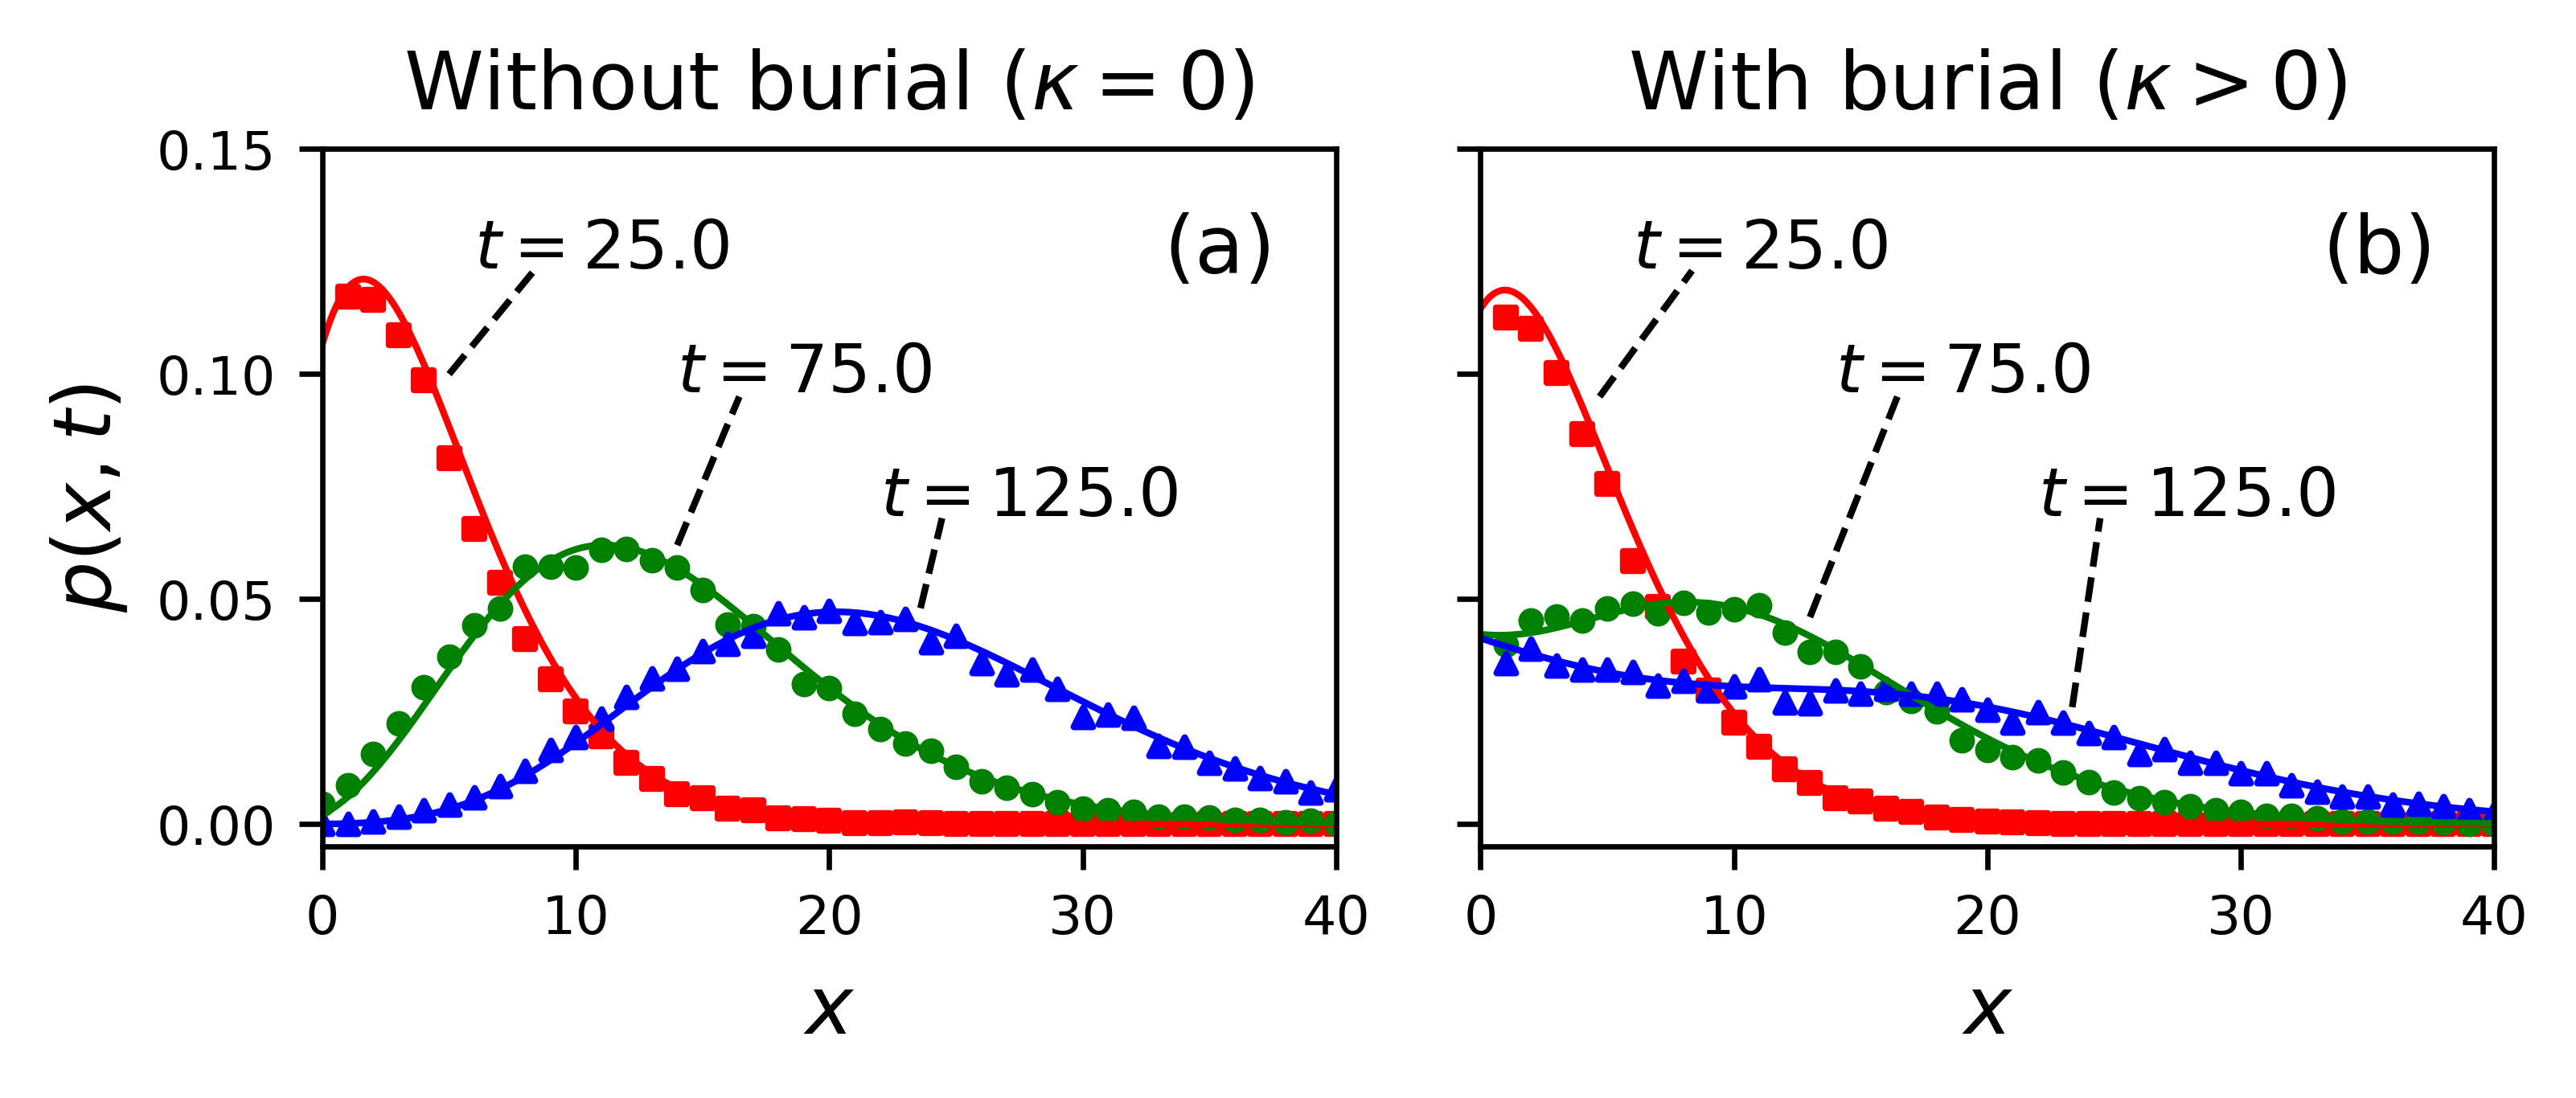
\includegraphics[width=\linewidth,keepaspectratio]{./figures/pdf-plot.png}
	\caption{Joint distributions for a grain to be at position $x$ at time $t$ are displayed for the choice $k_1=0.1$, $k_2=1.0$, $v=2.0$. Grains are considered initially at rest ($\theta_1=1$, $\theta_2=0$). The solid lines are the analytical distribution in equation (\ref{eq:pdf}), while the points are simulation results to show mathematical correctness. Colors pertain to different times. Units are unspecified, since our aim is to demonstrate the general characteristics of $p(x,t)$. Panel (a) shows the case $\kappa=0$ -- the absence of burial.
		In this case, the joint distribution tends toward Gaussian at large times \citep[e.g.][]{Einstein1937,Lisle1998}. Panel (b) shows the case when grains have rate $\kappa = 0.01$ to become buried while resting.
		Because of burial, the joint distribution tends toward a more uniform distribution than Gaussian. This shows a redistribution of probability to smaller values of $x$ due to the burial process \citep[cf.][]{Wu2019}. The redistribution is encoded mathematically by the Marcum Q-function terms in equation  (\ref{eq:pdf}). A similar tendency is seen in field studies of tracer dispersion in gravel bed rivers \citep[e.g.][]{Hassan1994}.}
	\label{fig:pdfs}
\end{figure}

% solution for case theta_1=1: distribution function
Using the propagators (\ref{eq:prop1}-\ref{eq:prop2}) and this transform calculus, the joint distribution $p(x,t)$ is derived in appendix \ref{sec:appendixA}, while the moments $\bra x \ket$ and $\bra x^2 \ket$ and ultimately the variance of position $\sigma_x^2(t)$ are derived in appendix \ref{sec:appendixB}. With the shorthand notations $\xi = k_2 x/v$, $\tau = k_1(t-x/v)$, and $\Omega = (\kappa+k_1)/k_1$ \citep[cf.][]{Lisle1998}, the joint distribution to find a grain at position $x$ at time $t$ is 
\begin{multline}
p(x,t) = \theta_1\mathcal{H}(\xi)\mathcal{H}(\tau)\Big[1-\frac{k_1}{\kappa+k_1}\Big(1-e^{-(\kappa+k_1)t}\Big)\Big]\delta(x) \\ + \frac{1}{v}e^{-\Omega \tau - \xi}\mathcal{H}(\xi)\mathcal{H}(\tau)\Big(\theta_1\Big[k_1\mathcal{I}_0\big(2\sqrt{\xi\tau}\big) + k_2\sqrt{\frac{\tau}{\xi}}\mathcal{I}_1\big(2\sqrt{\xi\tau}\big)\Big] \\ + \theta_2\Big[k_1\delta(\tau) + k_2 \mathcal{I}_0\big(2\sqrt{\xi\tau}\big)+k_1 \sqrt{\frac{\xi}{\tau}}\mathcal{I}_1\big(2\sqrt{\xi\tau}\big)\Big]\Big) \\
+ \frac{1}{v}\frac{\kappa k_2}{\kappa + k_1}e^{-\kappa \xi/(\kappa + k_1)}\mathcal{H}(\xi)\mathcal{H}(\tau)\Big[(\theta_1/\Omega)\mathcal{P}_2(\xi/\Omega,\Omega\tau) + \theta_2 \mathcal{P}_1(\xi/\Omega,\Omega\tau)\Big].
\label{eq:pdf}
\end{multline}
$\mathcal{H}$ is the Heaviside step function and we use the convention $\mathcal{H}(0)=1$.
The $\mathcal{I}_\nu$ are modified Bessel functions of the first kind, and the $\mathcal{P}_\mu$ are generalized Marcum Q-functions defined by $\mathcal{P}_\mu(x,y) = \int_0^y e^{-z-x}(z/x)^{(\mu-1)/2}\mathcal{I}_{\mu-1}(2\sqrt{xz})dz $ \citep{Temme1996}. Modified Bessel functions are common in one-dimensional diffusion problems \citep[e.g.][]{Einstein1937,Giddings1955,Daly2010}. 

The Marcum Q-functions are convolutions between modified Bessel functions and decaying exponentials. They were originally devised in relation to radar detection theory \citep{Marcum1960}. 
Conceptually, the Q-functions emerge in our context from the sediment burial process. According to our assumptions, resting grains can become buried in some interval of time with an exponential probability. Meanwhile, the probability that grains are resting follows a modified Bessel distribution \citep[e.g.][]{Einstein1937,Lisle1998}.
As a result, the probability that sediment is resting and becomes buried involves the convolution structure of the Marcum Q-functions.
Consistent with this interpretation, the terms involving these convolutions vanish when the burial rate is taken to zero $(\kappa \rightarrow 0)$.
Figure \ref{fig:pdfs} depicts the distribution (\ref{eq:pdf}) alongside simulations generated by a direct method based on evaluating the cumulative transition probabilities between states on a small timestep \citep[cf.][]{Barik2006}. A link to the simulation code, which includes descriptive comments, is available in the acknowledgments.



% solution for theta_1=1: moments
 The first two moments and the positional variance are derived in appendix \ref{sec:appendixB}.
The moments are
\begin{align}
\bra x(t) \ket &= A_1 e^{(b-a)t}+B_1e^{-(a+b)t}+C_1, \label{eq:mean}\\
\bra x^2(t) \ket &= A_2(t)e^{(b-a)t}+B_2(t)e^{-(a+b)t}+C_2. \label{eq:second}
\end{align}
In these equations, $a = (\kappa + k_1+k_2)/2$ and $b = \sqrt{a^2-\kappa k_2}$ are effective rates having dimensions of inverse time.
The $A_i$, $B_i$, and $C_i$ are polynomials available in table \ref{table:params}.
The variance is
\be \sigma_x^2(t) = A(t)e^{(b-a)t} + B(t)e^{-(a+b)t} + C(t). \label{eq:var}\ee
$A, B,$ and $C$ are transcendental functions available in table \ref{table:params}.
This equation represents the scale-dependence of bedload diffusion for sediment gradually undergoing burial.
\begin{table}[!h]
	\centering
	\caption{Polynomials and transcendental functions used in the expressions of the mean (\ref{eq:mean}), second moment (\ref{eq:second}) and variance (\ref{eq:var}) of bedload tracers.}
	\label{table:params}
	\begin{tabular}{c}
		\toprule
		$\begin{aligned}[t]
		&A_1 = \frac{v}{2b}\big[\theta_2+\frac{k_1+\theta_2\kappa}{b-a}\big] \\
		&B_1 = -\frac{v}{2b}\big[\theta_2-\frac{k_1+\theta_2 \kappa}{a+b}\big] \\
		&C_1 =  -\frac{v}{2b}\big[\frac{k_1+\theta_2 \kappa}{b-a}+\frac{k_1+\theta_2 \kappa}{a+b}\big]\\
		&A_2(t) = \frac{v^2}{2b^3}\Big[(bt-1)[k_1+\theta_2(2\kappa + k_1 + b-a)]+\theta_2b \\
		&\hspace{3cm} + \frac{(\kappa+k_1)(\theta_2\kappa+k_1)}{(b-a)^2}[(bt-1)(b-a)-b]\Big]\\
		&B_2(t) = \frac{v^2}{2b^3}\Big[(bt+1)[k_1 + \theta_2(2\kappa+k_1-a-b)]+\theta_2b\\
		&\hspace{3cm} -\frac{(\kappa+k_1)(\theta_2\kappa+k_1)}{(a+b)^2}[(bt+1)(a+b)+b]\Big]\\
		&C_2 = \frac{v^2}{2b^3}(\kappa+k_1)(\theta_2 \kappa + k_1)\Big[\frac{2b-a}{(b-a)^2}+\frac{a+2b}{(a+b)^2}\Big]\\
		&A(t) = A_2(t)-2A_1C_1 - A_1^2\exp[(b-a)t]\\
		&B(t) = B_2(t)-2B_1C_1 - B_1^2\exp[-(a+b)t]\\
		&C(t) = C_2-C_1^2-2A_1B_1\exp[-2at]\\			
		\end{aligned}$\\
		\bottomrule
	\end{tabular}
\end{table}

The positional variance is plotted in figure \ref{fig:var} for conditions $\theta_1=1$ and $k_2\gg k_1 \gg \kappa$.
We interpret "$\gg$" to mean "of at least an order of magnitude greater".
These conditions mean that all grains are initially at rest \citep[cf.][]{Wu2019}, motion intervals are typically much shorter than rests \citep[cf.][]{Einstein1937}, and sediment burial requires a much longer time than typical rests.
We concentrate on these conditions in this paper as they are most relevant to bedload diffusion in gravel-bed rivers, where sediment transport is typically rarefied and intermittent, and the burial process is relatively slow compared to surface resting times \citep[e.g.][]{Ferguson2002,Hassan1994}.
Figure \ref{fig:var} demonstrates that under these conditions the variance (\ref{eq:var}) shows three ranges of bedload diffusion with approximate power law scaling ($\sigma_x^2 \propto t^\gamma$), followed by a fourth range with no diffusion ($\sigma_x^2 = \text{const}$). We associate the first three ranges with the local, intermediate, and global ranges proposed by \citet{Nikora2001a,Nikora2002}, and identify the fourth range as resulting from the burial of all sediment grains.
We suggest to call the fourth range geomorphic, since any further transport in this range can occur only if scour exposes buried grains to the flow \citep[cf.][]{Nakagawa1980,Voepel2013,Martin2014}.
Using this terminology, we summarize when $k_2\gg k_1 \gg \kappa$ and $\theta_1=1$, the variance in equation (\ref{eq:var}) expresses four scaling ranges of bedload diffusion: local, intermediate, and global, and geomorphic.

\section{Discussion of scale-dependent bedload diffusion}
\label{sec:discussion}
\begin{figure}[t]	
	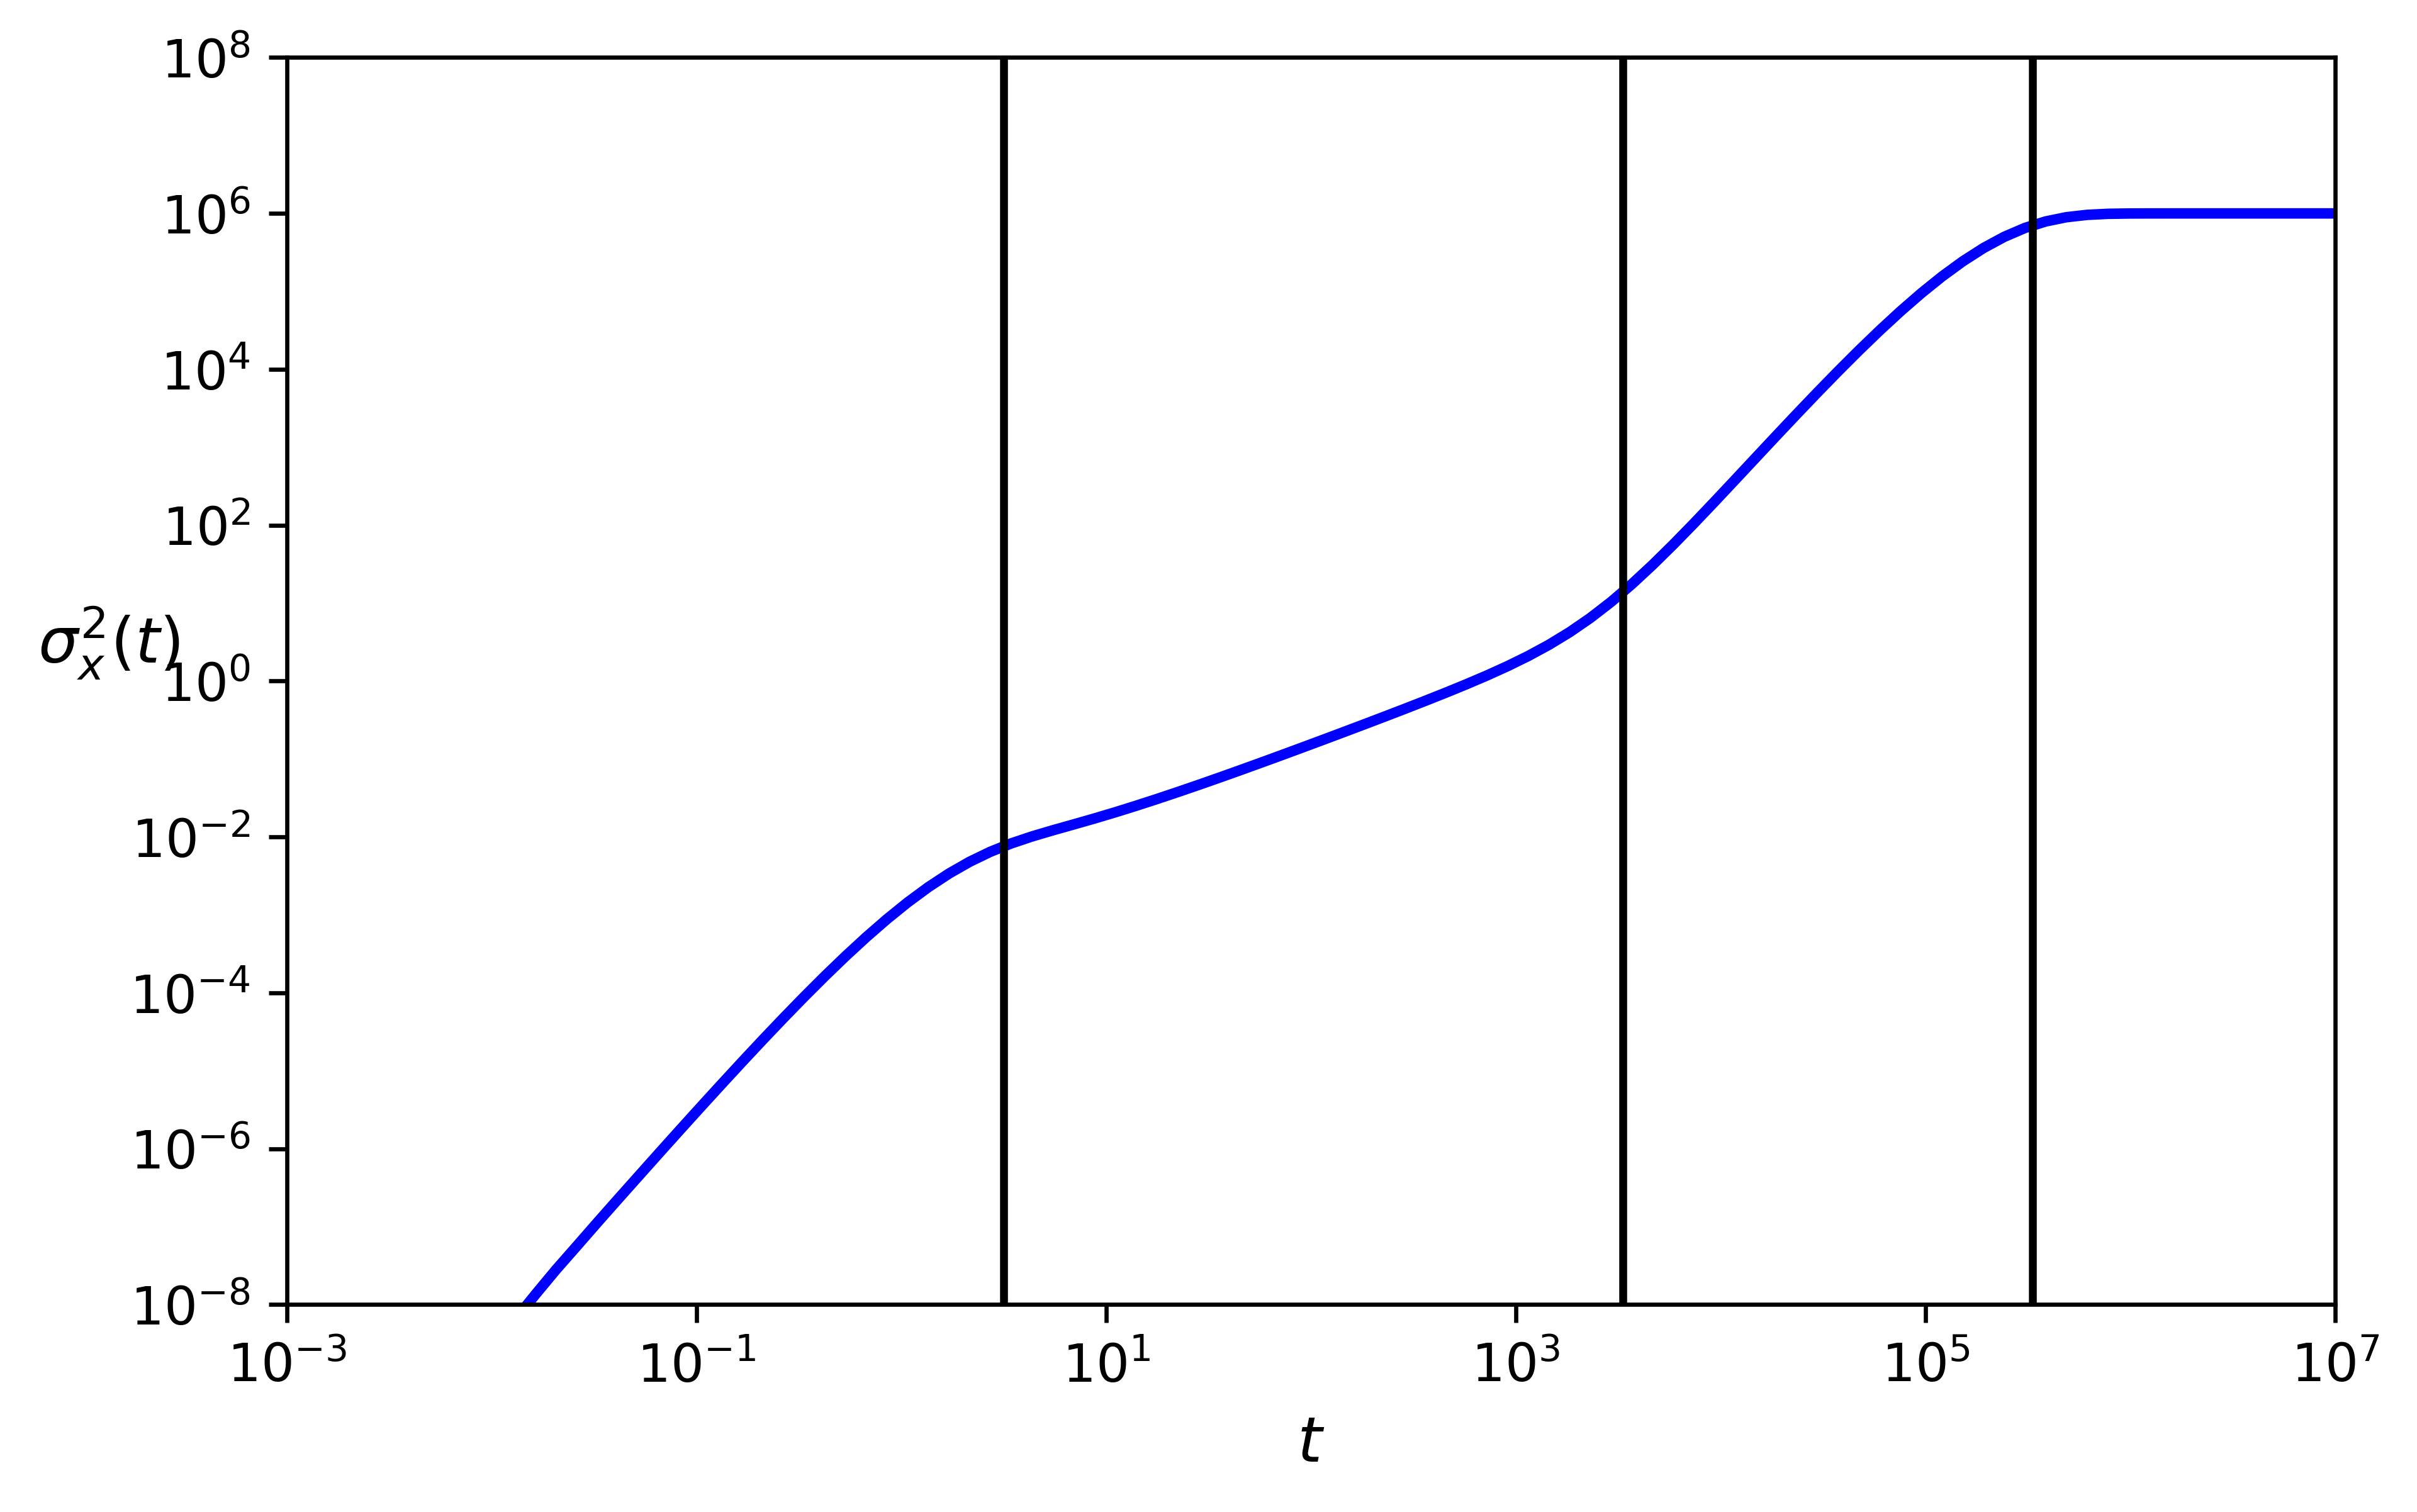
\includegraphics[width=\linewidth,keepaspectratio]{./figures/diffusion.png}
	\caption{The variance equation (\ref{eq:var}) is plotted for the parameters $1/k_2 = 1.5$s, $1/k_1 = 30.0$s, and $v=0.1$m/s. These values are comparable to laboratory flume experiments transporting small ($\sim 5$mm) gravels \citep[cf.][]{Lajeunesse2010,Martin2012}. The timescale of burial is set to $1/\kappa = 7200.0$s (two hours), and the initial condition is rest ($\theta_1=1$). The solid line is equation (\ref{eq:var}) while the points are directly simulated. When $k_2\gg k_1 \gg \kappa$, as as is the case in this plot, there are four distinct scaling ranges of $\sigma_x^2$: local, intermediate, global, and geomorphic. Within each range, a slope key is added to demonstrate the scaling $\sigma_x^2 \propto t^\gamma$. There are three crossovers between these ranges, denoted on the figure by vertical lines. Crossover times $T_L$, $T_I$, and $T_G$ are indicated at the bottom of the plot. They are given in equations (\ref{eq:TL}-\ref{eq:TG}) in terms of the model's input parameters. }
	\label{fig:var}
\end{figure}

The model we've presented involves four parameters. These are the characteristic velocity $v$ of moving sediment and three key timescales: $1/k_2$, $1/k_1$, and $1/\kappa$.
The timescales represent the mean duration of motion, the mean duration of rest, and the mean duration of rest before burial occurs.
As shown in figure \ref{fig:var}, scaling laws $\sigma_x^2 \propto t^\gamma$ approximately characterize the diffusion in each scaling range.
The exponents $\gamma$ in each range result from competition between different terms in equation (\ref{eq:var}).
Between these ranges, there are crossover regions where the scaling is not a simple power law.
Because these crossover regions are relatively narrow, we can approximately characterize them with crossover times $T_L$, $T_I$, and $T_G$.
These times partition the diffusion ranges into $0< t < T_L$ (local), $T_L < t < T_I$ (intermediate), $T_I < t < T_G$ (global), and $T_G < t$ (geomorphic). 
Figure \ref{fig:var} depicts these crossover times as vertical lines.
To understand the scale dependence expressed by the bedload variance in equation (\ref{eq:var}), we need to determine the exponents $\gamma$ of each range and relate the crossover times $T_L$, $T_I$, and $T_G$ between diffusion ranges to the model parameters $v$, $k_1$, $k_2$, and $\kappa$.

% now we figure out what the exponents are 
We determine the diffusion exponents $\gamma$ in the local, intermediate, and global ranges using two limiting cases of equation (\ref{eq:var}): (1) $t\ll 1/\kappa$, and (2) $1/k_2 \rightarrow 0$ while $vk_2 = \text{const}$.
Limit (1) corresponds to times so short a negligible amount of sediment burial has occurred, while limit (2) corresponds to times so long a motion interval appears as an instantaneous step having mean step length $l=vk_2$.
We evaluate these limits in appendix \ref{sec:appendixC} and obtain the diffusion exponents.
Local range diffusion has exponent $2 \leq \gamma \leq 3$ depending on the initial conditions $\theta_1$ and $\theta_2$.
When the initial conditions are pure, meaning one of the $\theta_i$ is zero, the local exponent is $\gamma=3$.
When grains start in a mixture of motion and rest states, meaning neither $\theta_i$ is zero, the local exponent is $\gamma=2$.
Intermediate range diffusion always has exponent $\gamma=1$, agreeing with the classic flume experiments based on visually tracking painted sediment \citep[e.g.][]{Einstein1937,Yano1969a,Nakagawa1976}.
Finally, global range diffusion has exponent $1 < \gamma < 3$ depending on the ratio $k_1/\kappa$.
In the extreme case $k_1/\kappa \approx 0 $, we find normal diffusion $\sigma_x^2 \propto t$. 
However, in the opposite extreme $k_1/\kappa \rightarrow \infty$, we find  super-diffusion $\sigma_x^2 \propto t^3$.
For general values of the ratio $\kappa/k_1$, the global exponent lies between these extremes.
For the parameters generating figure \ref{fig:var}, the global range exponent is $\gamma \approx 2.2$. 
We surmise when the model parameters satisfy $k_2\gg k_1 \gg \kappa$ meaning all three diffusion ranges exist, the variance (\ref{eq:var}) implies local range super-diffusion with exponent depending on the $\theta_i$, intermediate range normal diffusion with no dependence on model parameters, and global range super-diffusion with exponent depending on the ratio $k_1/\kappa$.
Finally, the model supports a geomorphic range of no diffusion ($\gamma=0$) associated with the eventual and permanent trapping of all sediment grains.

Each of the three crossover times relates to a physical process affecting a population of grains.
Exchange between motion and rest states induces the local/intermediate crossover, the onset of sediment burial induces the intermediate/global crossover, and the completion of sediment burial induces the global/geomorphic crossover.
Each process admits two characteristic times, and we formulate the crossover times heuristically as geometric averages of these characteristic times:
\begin{alignat}{2}
&T_L &&= \sqrt{\frac{1}{k_1}\frac{1}{k_2}}, \label{eq:TL}\\
&T_I &&= \sqrt{\frac{1}{k_1}\frac{1}{\kappa}},\label{eq:TI}\\
&T_G &&= \sqrt{\frac{1}{\kappa}\frac{k_1+k_2}{\kappa k_1}} \label{eq:TG}.
\end{alignat}
Figure \ref{fig:var} depicts these relationships as dashed vertical lines.
The times $1/k_1$ and $1/k_2$ characterize exchanges between motion and rest, while $1/k_1$ and $1/\kappa$ characterize the onset of burial originating from grains buried in their first resting sojourns.
Equations (\ref{eq:TL}) and (\ref{eq:TI}) mix these paired times.
The completion of sediment burial and its characteristic timescales originate from the last grains to bury.
In one extreme, all grains rest on the surface, meaning the last grains bury around $1/\kappa$; while in another, a fraction of grains remains in motion for a long time evading burial.
By analogy to the mobile-immobile model of \citet{Ancey2006}, we reason that a fraction $k_1/(k_1+k_2)$ of the free population will be in motion and evading burial at long timescales, and for this fraction we propose an effective trapping rate $\kappa k_1/(k_1+k_2)$.
Equation (\ref{eq:TG}) mixes the reciprocal of this effective rate with $1/\kappa$.
We tested formulas (\ref{eq:TL}-\ref{eq:TG}) for many parameter choices and conclude they adequately represent the crossover locations between diffusion regimes provided the parameters satisfy $k_2\gg k_1 \gg \kappa$ and grains start from rest ($\theta_1=1$).
However, starting grains from motion ($\theta_2=1$) widens the crossover region between local and intermediate ranges, meaning equation (\ref{eq:TL}) loses representative power; while setting relatively very large values of $k_2$ widens the crossover region between global and geomorphic ranges, meaning equation (\ref{eq:TG}) loses representative power.
Ultimately, we emphasize the representation of finite width crossover regions by crossover times is an idealization, so we propose equations (\ref{eq:TL}-\ref{eq:TG}) as heuristics. 
These relations provide useful divisions between the bedload diffusion scaling ranges.

In this letter, we have developed a model extending earlier works to describe four ranges of bedload diffusion.
The model reduces to earlier works through the two simplified limits previously leveraged to extract the scaling exponents $\gamma$.
As discussed in appendix \ref{sec:appendixC}, limit (1) implies the model developed by \citet{Lisle1998} to describe soil transport within a sheet flow, while limit (2) implies the model developed by \citet{Wu2019} to describe bedload transport with burial burial.
Either of these cases further simplifies to the classic results of \citet{Einstein1937} and his early followers \citep[e.g.][]{Hubbell1964, Nakagawa1976, Yano1969} predicting a single range of normal diffusion.
\citet{Lisle1998} generalized the Einstein model to include a finite velocity and duration of motion in place of instantaneous steps, and they derived two ranges of diffusion -- super-diffusive and normal.
\citet{Wu2019} developed an active layer formulation of bedload transport where grains are transferred from the active layer (surface) to the substrate layer (burial) at a constant rate.
They simplified the problem by interpreting motions as instantaneous steps and derived two ranges of diffusion -- normal and super-diffusive.
Our model ultimately extends these two works and re-frames them in the formalism of CTRWs \citep[e.g.][]{Weiss1994} that was implicitly applied by \citet{Einstein1937}.

We offer several implications of our model for bedload diffusion studies in gravel-bed streams.
First, our model confines the valid range of scale-independent models such as the advection-diffusion equation \citep[e.g.][]{Ganti2010} and the Einstein model \citep[e.g.][]{Martin2012} for practical applications such as contaminant transport \citep[e.g][]{Malmon2005,Macklin2006} and aquatic habitat restoration \citep[e.g.][]{Gaeuman2017}.
We can conclude when the observation timescale satisfies $T_L<t<T_I$, with $T_L$ and $T_I$ given by equations (\ref{eq:TL}) and (\ref{eq:TI}), we expect normal bedload diffusion $\sigma_x^2 = D_d t$.
Second, the model links bedload transport understanding across scales. 
In practice, we might measure sediment diffusion within a channel on one timescale with intent to apply our knowledge at smaller or larger timescales; usually, experimental limitations constrain the measurement timescale.
For example, we could determine $k_1$ and $k_2$ by measuring the virtual velocity and diffusivity of sediment tracers in the intermediate range \citep[e.g.][]{Einstein1937,Yano1969a,Nakagawa1976}, although experimental limitations complicate determinations of global range characteristics.
With an estimate of the trapping rate $\kappa$, equation (\ref{eq:var}) provides diffusion characteristics of the global range $T_I<t<T_G$ which is more difficult to study experimentally.

Finally, we highlight some limitations of our model and propose topics for further research.
Two issues are our treatment of sediment burial as a permanent condition and  our implicit assumption that burial is the only trapping process affecting grains.
In actuality, burial is a temporary condition linked to scour and fill of the sedimentary bed \citep{Hassan1994,Ferguson2002a,Voepel2013,Martin2014}, and other processes trap sediment in field experiments: for example, water depth changes can strand sediment on bars and floodplains \citep[e.g.][]{Ferguson2002a, Bradley2017, Malmon2003}.
In principle, the multi-state CTRW framework we used here can describe bedload diffusion with multiple trapping processes by simply adding more states, and it can handle impermanent sojourns in these states by specifying propagators for them.
However, we currently lack the experimental knowledge to specify these propagators, since trapping rates and durations are poorly understood.
For example, recent experiments have attributed resting times to any non-moving sediment, whether trapped or not, and this is known to imply heavy-tailed sediment resting time distributions \citep[e.g.][]{Olinde2015,Bradley2017}.
However, very few experimental studies have resolving the immobile times of sediment while accounting for their mechanism \citep[e.g.][]{Martin2014}.
We propose experiments to determine the rates and durations of specific bedload trapping processes are important topics for further study.
A first step might be to measure the burial rate $\kappa$ we applied in this letter; in principle, this could be discerned by timing the period required for tagged surface grains to become buried in flumes.
Ultimately, we envision leveraging an improved understanding of rates and durations of sediment trapping processes to develop a link between grain-scale and geomorphic processes in river channels.

\section{Conclusion}
\label{sec:conclusion}
We have developed a random walk model between alternating mobile and immobile states having a possibility of trapping from the immobile state, and we have used it to describe the diffusion of bedload sediment transporting through a river channel as it gradually becomes buried.
This ultimately extends the original diffusion model of \citet{Einstein1937}.
To our knowledge, this model is the first analytical description of bedload diffusion across the local, intermediate, and global timescales introduced by \citet{Nikora2001a}.
Pushing the ideas of Nikora et al. somewhat further, we have proposed a geomorphic range to describe diffusion characteristics at timescales larger than the global range.
These timescales will involve morphodynamic processes in their description.
At base level, our model shows the essential ingredients of three diffusion stages: (1) the duration of sediment motions, (2) mobile-immobile switching, and (3) a trapping process.
A next step from our work is to incorporate the bed scour process that re-exposes buried sediment. 
This will better resolve the diffusion characteristics of the global and geomorphic ranges.
Ultimately, we advocate keeping the multi-state random walk formalism from physics close, as we believe it implicitly underlies most existing bedload diffusion works and should readily accommodate extensions aimed at incorporating more physical processes into Einstein's research paradigm.

\appendix

\section{Calculation of the distribution function}
\label{sec:appendixA}
Double transforming (\ref{eq:x}-\ref{eq:y}) using the definition (\ref{eq:doubletransform}) gives

\begin{alignat}{2}
&\tom_{1T}(\eta,s) &&= \theta_1 \tg_1(\eta,s) + \tom_2(\eta,s)\tg_1(\eta,s)-\tom_{1F}(\eta,s),\\
&\tom_{1F}(\eta,s) &&= \theta_1\tg_1(\eta,s+\kappa) + \tom_2(\eta,s)\tg_1(\eta,s+\kappa),\\
&\tom_2(\eta,s) &&= \theta_2 \tg_2(\eta,s) + \tom_{1F}(\eta,s)\tg_2(\eta,s).
\end{alignat}
This purely algebraic system solves for 
\begin{alignat}{2}
&\tom_{1T}(\eta,s) &&= \frac{\theta_1 + \theta_2 \tg_2(\eta,s)}{1-\tg_1(\eta,s+\kappa)\tg_2(\eta,s)}\big\{\tg_1(\eta,s)-\tg_1(\eta,s+\kappa) \big\}, \label{eq:A} \\
&\tom_{1F}(\eta,s) &&= \frac{\theta_1 + \theta_2 \tg_2(\eta,s)}{1-\tg_1(\eta,s+\kappa)\tg_2(\eta,s)}\tg_1(\eta,s+\kappa),\\
&\tom_{2}(\eta,s) &&= \frac{\theta_2 + \theta_1 \tg_1(\eta,s+\kappa)}{1-\tg_1(\eta,s+\kappa)\tg_2(\eta,s)}\tg_2(\eta,s). 
\end{alignat}
Double transforming (\ref{eq:b}-\ref{eq:z}) gives
\begin{align}
\tp_0(\eta,s) &= \frac{1}{s}\tom_{1T}(\eta,s),\\
\tp_1(\eta,s) &= \theta_1 \tG_1(\eta,s) + \tom_2(\eta,s) \tG_1(\eta,s),\\
\tp_2(\eta,s) &= \theta_2 \tG_2(\eta,s) + \tom_{1F}(\eta,s)\tG_2(\eta,s).\label{eq:Z}
\end{align}
The total probability is $p(x,t) = p_0(x,t) + p_1(x,t) + p_2(x,t)$. Using equations (\ref{eq:A}-\ref{eq:Z}) this becomes, in the double Laplace representation, 
\begin{multline}
\tp(\eta,s) = \frac{1}{s}\frac{\theta_1 + \theta_2 \tg_2(\eta,s)}{1-\tg_1(\eta,s+\kappa)\tg_2(\eta,s)}\big\{\tg_1(\eta,s)-\tg_1(\eta,s+\kappa) \big\} \\
+\frac{\theta_1\big[\tG_1(\eta,s) + \tg_1(\eta,s+\kappa)\tG_2(\eta,s)\big]+ \theta_2\big[\tG_2(\eta,s) + \tg_2(\eta,s)\tG_1(\eta,s)\big]}{1-\tg_1(\eta,s+\kappa)\tg_2(\eta,s)}. \\
\label{eq:lap}
\end{multline}
Plugging the propagators outlined in equations (\ref{eq:prop1}-\ref{eq:prop2}) into equation (\ref{eq:lap}) gives 
\be \tilde{p}(\eta,s) = \frac{1}{s}\frac{(s+\kappa + k')s  + \theta_1(s+\kappa )\eta v+ \kappa k_2}{(s+\kappa+k_1)\eta v+(s+\kappa+k')s + \kappa k_2}.\label{eq:nicedist}\ee
In this equation, $k'=k_1+k_2$, and we have used the normalization requirement of the initial probabilities $\theta_1 + \theta_2 = 1.$
The double inverse transform of this equation provides the distribution $p(x,t)$.
It is convenient to invert the transform over $\eta$ first.
Using the results 15.103 (transform of exponential), 15.123 (transform of derivative), and 15.141 (transform of Dirac delta function) from \citet{Arfken1985} provides 
\begin{multline} \tp(x,s) = \theta_1 \frac{s+\kappa}{s(s+\kappa + k_1)}\delta(x) + \frac{1}{v} \Big(\frac{(s+\kappa+k')s+\kappa k_2}{s(s+\kappa+k_1)} \\- \frac{\theta_1(s+\kappa)[s(s+\kappa+k_1)+\kappa k_2]}{s(s+\kappa+k_1)^2}\Big)
\exp\Big[-\frac{(s+\kappa+k')s+\kappa k_2}{s+\kappa+k_1}\frac{x}{v}\Big].\end{multline}
Taking the remaining inverse transform over $s$, applying results 15.152 (substitution), 15.164 (translation), and 15.175 (transform of $te^{kt}$) from \citet{Arfken1985}, and defining the shorthand notations $\tau = k_1(t-x/v)$, $\xi = k_2 x/v$, and $\Omega = (\kappa + k_1)/k_1$, gives the simpler form 
\begin{multline}
p(x,t) = \theta_1\Big[1-\frac{k_1}{\kappa + k_1}\big(1-e^{-(\kappa + k_1)t}\big)\Big]\delta(x) + \frac{1}{v}\exp[\Omega \tau - \xi]\\
\times \El^{-1}\Big\{\Big( \theta_2 + \frac{\theta_1k_1+\theta_2 k_2}{s}+\frac{\theta_1k_1k_2}{s^2} + \frac{\theta_2\kappa k_2}{s(s-\kappa-k_1)} + \frac{\theta_1\kappa k_1 k_2}{s^2(s-\kappa-k_1)}\Big)\\
\times\exp\big[\frac{k_1 \xi}{s}\big];\tau/k_1\Big\}.
\end{multline}
Using entries 2.2.2.1, 2.2.2.8, and 1.1.1.13 from \citet{Prudnikov1992a} in conjunction with the definition of the Marcum Q-function $ \mathcal{P}_\mu(x,t)$ \citep[e.g.][]{Temme1996}, and inserting the Heaviside functions to account for the fact that grains can neither travel backwards nor at speeds exceeding $v$, we finally arrive at equation \ref{eq:pdf} for the joint distribution $p(x,t)$.

\section{Calculation of the moments}
\label{sec:appendixB}
We leverage equation \ref{eq:momenttrick} to compute the first two moments of position $x$ and ultimately its variance. The first two derivatives of the double Laplace transformed distribution (\ref{eq:nicedist}) are
\be \partial_\eta \tp(\eta,s) = -v \frac{1}{s}\frac{[(s+\kappa + k')s + \kappa k_2][\theta_2(s+\kappa) + k_1]}{[\eta v(s+\kappa +k_1) + (s+ \kappa + k')s+\kappa k_2]^2},\ee
\be \partial_\eta^2 \tp(\eta,s) = 2v^2 \frac{1}{s} \frac{(s+\kappa+k_1)[(s+\kappa + k')s+\kappa k_2][\theta_2(s+\kappa) + k_1]}{[\eta v(s+\kappa + k_1) + (s+\kappa + k')s+ \kappa k_2]^3}.\ee
Evaluating these at $\eta=0$ and applying equation (\ref{eq:momenttrick}) provides the Laplace transformed moments
\be  \frac{\bra\tilde{x}(s)\ket} {v} = \frac{1}{s}\frac{\theta_2(s+\kappa)+k_1}{(s+\kappa+k')s+\kappa k_2} = \frac{1}{s} \frac{\theta_2(s+\kappa)+k_1}{(s+a+b)(s+a-b)}\label{eq:lapmean},\ee
\be \frac{\bra \tilde{x}^2(s) \ket}{2v^2} = \frac{1}{s} \frac{(s+\kappa+k_1)(\theta_2(s+\kappa)+k_1)}{[(s+\kappa+k')s+\kappa k_2]^2}=  \frac{1}{s}\frac{(s+\kappa+k_1)(\theta_2(s+\kappa)+k_1)}{(s+a+b)^2(s+a-b)^2}.\label{eq:lapsecondmom}\ee
The parameters $a= (\kappa+k')/2$ and $b^2 = a^2 -\kappa k_2$ were introduced to factorize the denominators.
These equations can be inverted using the properties 15.164 (translation), 15.11.1 (integration), and 15.123 (differentiation) from  \citet{Arfken1985} after expansion in partial fractions.
For the mean, the calculation is
\begin{align}
\frac{2b}{v}\bra x \ket &= \big[\theta_2 + (k_1+\theta_2 \kappa)\int_0^t dt\big]\El^{-1}\Big\{ \frac{1}{s+a-b}-\frac{1}{s+a+b};t\Big\}\\
&= \Big[\theta_2 + \frac{k_1+\theta_2\kappa}{b-a}\Big]e^{(b-a)t} - \Big[\theta_2 - \frac{k_1+\theta_2\kappa}{a+b}\Big]e^{-(a+b)t} - \Big[\frac{k_1+\theta_2\kappa}{b-a} + \frac{k_1+\theta_2\kappa}{a+b}\Big].
\end{align}
This equation rearranges to (\ref{eq:mean}).
The second moment (\ref{eq:lapsecondmom}) is 
\begin{multline}
\frac{2b^2}{v^2}\bra x^2 \ket = \Big[\theta_2(\delta(t) + \partial_t) + (\theta_2(2\kappa + k_1)+k_1) + (\kappa+k_1)(\theta_2\kappa+k_1)\int_0^t dt \Big] \\
\times \El^{-1}\Big\{ \frac{1}{(s+a-b)^2} + \frac{1}{(s+a+b)^2}-\frac{1}{b(s+a-b)}+\frac{1}{b(s+a+b)};t\Big\}.
\end{multline}
This becomes 
\begin{multline}
\frac{2b^3}{v^2}\bra x^2 \ket = \Big[\theta_2\partial_t + [\theta_2(2\kappa+k_1)+k_1] + (\kappa+k_1)(\theta_2\kappa+k_1)\int_0^tdt\Big]\\
\times \Big((bt-1)e^{(b-a)t}+(bt+1)e^{-(a+b)t}\Big),
\end{multline}
which evaluates to equation (\ref{eq:second}).
$\sigma_x^2 = \bra x^2 \ket - \bra x \ket^2$ derives the variance in equation (\ref{eq:var}).

\section{Limiting behavior of the moments}
\label{sec:appendixC}
Taking two limits of the variance in equation (\ref{eq:var}) reveals the diffusion exponents $\gamma$ of each range and links our model to the earlier works of \cite{Wu2019}, \citet{Lisle1998}, and ultimately \citet{Einstein1937}.
The first limit neglects the burial process $(\kappa \rightarrow 0$) but retains the finite velocity and motion duration in equations (\ref{eq:lapmean}) and (\ref{eq:lapsecondmom}).
The second limit sends the mean duration of motion to zero ($1/k_2\rightarrow 0$) and the velocity to infinity ($v\rightarrow \infty$) while holding the mean step distance $l = v/k_2$ constant.
In both cases, we mostly use the initial condition that grains start at rest ($\theta_1=1$).
The easiest approach to find the limiting form of the positional variance is to use the Laplace transformed moments (\ref{eq:lapmean}) and (\ref{eq:lapsecondmom}) as the starting point.

The first limit characterizes the local and intermediate ranges, since it concentrates on scales where the burial has not yet had time to occur. 
Taking $\kappa \rightarrow 0$ in equations (\ref{eq:lapmean}) and (\ref{eq:lapsecondmom}) with initial condition $\theta_1=1$ provides
\begin{align}
\bra \tilde{x} \ket &= vk_1 \frac{1 }{s^2(s+k')}, \label{eq:li1}\\
\bra \tilde{x}^2 \ket &= 2v^2k_1 \frac{s+k_1}{s^3(s+k')^2}. \label{eq:li2}
\end{align}
Inverting these equations provides the variance
\be \sigma_x^2 = 2v^2\frac{k_1}{k'^4}\Big(k_1\big[\frac{1}{2} - k'te^{-k't} - \frac{1}{2} e^{-2k't}\big] + k_2\big[-2+k't + (2+k't)e^{-k't}\big]\Big).\label{eq:li}\ee
This result encodes two stages of diffusion and can also be derived from the governing equations of the \citet{Lisle1998} model.
Expanding for small $t$ provides $\sigma_x^2(t) = v^2k_1t^3/3$ -- local range super-diffusion.
Expanding for large $t$ provides $\sigma_x^2(t) = 2v^2k_1k_2t/k'^3$ -- intermediate range normal diffusion.
Finally, we analyze this limit for arbitrary initial conditions to highlight the effect of initial conditions on the local range superdiffusion.
By applying Tauberian theorems, we can argue the $ t \rightarrow 0$ variance is determined by the $s\rightarrow \infty$ limits of (\ref{eq:lapmean}) and (\ref{eq:lapsecondmom}) \citep[e.g.][]{Weiss1994, Weeks1998}.  Expanding these equations in powers of $1/s \ll 1$ and inverting the resulting transforms gives
\begin{align} \bra x \ket &= v \theta_2 t + \frac{1}{2}v(\theta_1k_1-\theta_2k_2)t^2 + O(t^3),\\
\bra x^2 \ket &= v^2\theta_2 t^2 + \frac{1}{3}v^2(\theta_1k_1-2\theta_2k_2)t^3+ O(t^4).
\end{align}
This equation shows the effect of initial conditions on the diffusion characteristics of the local range:
\be \sigma_x^2(t) \sim v^2\theta_1\theta_2t^2 + \frac{1}{3}v^2(\theta_1k_1+\theta_2k_2)t^3.\label{eq:init}\ee
We have taken only leading order terms for any options of $\theta_1$ and $\theta_2$.
Equation (\ref{eq:init}) shows local range exponent $\gamma=2$ when initial conditions are mixed (both non-zero) and $\gamma=3$ when initial conditions are pure (one zero). Equation (\ref{eq:li}) shows intermediate range exponent $\gamma=1$.
These conclusions are characteristic of the \citet{Lisle1998} work while somewhat extending their analysis.
Finally, we note without showing it that all of these results further reduce to the \citet{Einstein1937} model in the limit of instantaneous steps: $1/k_2 \rightarrow 0$ and $v\rightarrow \infty$ while $v/k_2 = l$.

The second limit characterizes the intermediate, global, and geomorphic ranges, since it concentrates on scales where the duration of motion appears negligible.
Taking $1/k_2 \rightarrow 0$ and $v\rightarrow \infty$ while $v/k_2 = l$ in  equations (\ref{eq:lapmean}) and (\ref{eq:lapsecondmom}) provides
\begin{align}
\bra \tilde{x} \ket &= k_1l\frac{1}{s(s+\kappa)},\\
\bra \tilde{x}^2 \ket &= 2l^2k_1 \frac{s+\kappa+k_1}{s(s+\kappa)^2}.
\end{align}
Inverting these equations and introducing the variables $c=lk_1$ (an effective velocity) and $D_d = l^2k_1$ (a diffusivity) provides positional variance
\be \sigma_x^2(t) = \frac{2D_d(1-e^{-\kappa t})}{\kappa} + \frac{(1-e^{-2\kappa t}-2e^{-\kappa t}\kappa t)c^2}{\kappa^2}. \label{eq:wuvar}\ee
This is mathematically identical to the key result of \citet{Wu2019}.
Expanding for small $t$ provides $\sigma_x^2(t) = 2D_d t$ -- an intermediate range normal diffusion, while sending $t\rightarrow \infty$ provides $\sigma_x^2 = (2D_d\kappa + c^2)/\kappa^2$ -- a constant variance in the geomorphic range.
The global range is characterized by competition between both terms in \ref{eq:wuvar}, and shows $2 \leq \gamma \leq 3$ depending on the ratio $k_1/\kappa$ \citep[cf.][]{Wu2019}.
Finally, we note the further limit $\kappa \rightarrow 0$ produces $\sigma_x^2(t) = 2D_d t$.
This is the original result of \citet{Einstein1937} and represents a single range of normal diffusion \citep[e.g.][]{Hubbell1964,Nakagawa1976}.
The limits analyzed in this appendix ultimately support the arguments in section \ref{sec:discussion}.

\acknowledgments
J. Pierce acknowledges helpful exchanges with Eduardo Daly and Peter H{\"a}nggi during the early stages of this work. He would like to thank Melinda Saunders and Leonardo Golubovic for their careful guidance in mathematics through the years. M. Hassan is supported by an NSERC Discovery grant. The Python simulation code is available at \sloppy
\url{https://github.com/kevinkayaks/rw-diffu}.

\bibliography{biblio.bib}
\end{document}